\chapterimage{orange2.jpg} % Chapter heading image
\chapterspaceabove{6.75cm} % Whitespace from the top of the page to the chapter title on chapter pages
\chapterspacebelow{7.25cm} % Amount of vertical whitespace from the top margin to the start of the text on chapter pages

\chapter{Lyapunov Stability II: Nonautonomous Systems}\index{Lyapunov Stability II: Nonautonomous Systems}

\section{Overview}\index{Overview}
In the previous chapter, we studied autonomous systems, where the dynamics depend only on the state variables. We now extend the discussion to \textbf{nonautonomous systems}, where time explicitly appears as a second variable in the system dynamics. Such systems are represented as
\[
\dot{x}(t) = f(x,t), \quad x \in \mathbb{R}^n, \; t \in \mathbb{R}.
\]

The presence of time makes the analysis more challenging, since the system’s behavior may vary depending on when an input or disturbance is applied. For example, equilibrium points can shift or even cease to exist in the classical sense, and stability must be understood relative to a time-varying reference.

In this chapter, we adapt Lyapunov’s direct method to nonautonomous systems by introducing \textbf{Lyapunov functions with explicit time dependence} \( V(x,t) \). This allows us to study stability notions such as \textit{uniform stability}, \textit{uniform asymptotic stability}, and \textit{exponential stability}, which are crucial in time-varying and control-driven systems.

This framework broadens the applicability of Lyapunov’s theory, enabling the analysis of systems with time-varying parameters, switching dynamics, and external inputs---common in modern control applications.

%------------------------------------------------
\section{Definitions}\index{Definitions}

\begin{definition}[Stability Concepts]
Consider the system $\dot{x}=f(x,t)$ with equilibrium $x=0$.  
\begin{itemize}
    \item \textbf{Stable:} For every $\epsilon>0$ and $t_0$, there exists $\delta(\epsilon,t_0)>0$ such that
    \[
    ||x(t_0)|| < \delta \;\; \Rightarrow \;\; ||x(t)|| < \epsilon, \quad \forall t \geq t_0.
    \]
    \item \textbf{Convergent:} $x(t) \to 0$ as $t \to \infty$.
    \item \textbf{Asymptotically Stable:} The equilibrium is stable and convergent.  
    \item \textbf{Unstable:} The equilibrium is not stable.  
\end{itemize}
\end{definition}

\begin{definition}[Uniform Stability Concepts]
The equilibrium $x=0$ is said to be uniformly stable if the $\delta$ in the stability definition is independent of $t_0$.  
\begin{itemize}
    \item \textbf{Uniformly Stable:} $\delta = \delta(\epsilon)$ independent of $t_0$.  
    \item \textbf{Uniformly Convergent:} For every $\epsilon>0$, there exists $T(\epsilon)>0$ independent of $t_0$ such that
    \[
    t \geq t_0 + T(\epsilon) \;\; \Rightarrow \;\; ||x(t)|| < \epsilon.
    \]
    \item \textbf{Uniformly Asymptotically Stable (UAS):} Uniformly stable and uniformly convergent.  
    \item \textbf{Globally Uniformly Asymptotically Stable (GUAS):} Uniformly asymptotically stable with region of attraction $\mathbb{R}^n$.  
\end{itemize}
\end{definition}

\begin{definition}[Exponential Stability]
The equilibrium $x=0$ is \textbf{exponentially stable} if there exist constants $\alpha>0$, $\lambda>0$, and $\delta>0$ such that
\[
||x(t)|| \leq \alpha \, ||x(t_0)|| e^{-\lambda (t-t_0)}, \quad \forall t \geq t_0, \; ||x(t_0)|| < \delta.
\]
If the inequality holds for all $x(t_0)\in\mathbb{R}^n$, the equilibrium is \textbf{globally exponentially stable}.
\end{definition}

%------------------------------------------------
\section{Positive Definite Functions}\index{Positive Definite Functions}

Let $W : D \times \mathbb{R}^+ \to \mathbb{R}$ be a scalar function, where $D \subseteq \mathbb{R}^n$ is a domain containing the origin.  
Assume that $W(x,t)$ is continuous in $(x,t)$ and has continuous partial derivatives with respect to $x$.

\begin{definition}[Positive Semi-Definite Function]
A function $W(x,t)$ is said to be \textbf{positive semi-definite} in $D$ if
\[
W(0,t) = 0 \forall t \in \mathbb{R}^+
\]
\[
W(x,t) \geq 0, \quad \forall (x,t) \in D \times \mathbb{R}^+.
\]
\end{definition}

\begin{definition}[Positive Definite Function]
A function $W(x,t)$ is said to be \textbf{positive definite} in $D$ if
\[
W(0,t) = 0, \quad W(x,t) > 0 \;\; \forall x \neq 0,
\]
and there exists a continuous function $V_1(x)$ with $V_1(0)=0$ such that
\[
V_1(x) \leq W(x,t), \quad \forall (x,t) \in D \times \mathbb{R}^+.
\]
\end{definition}

\begin{definition}[Decrescent Function]
A function $W(x,t)$ is said to be \textbf{decrescent} in $D$ if there exists a continuous function $V_2(x)$ with $V_2(0)=0$ such that
\[
W(x,t) \leq V_2(x), \quad \forall (x,t) \in D \times \mathbb{R}^+.
\]
\end{definition}

\begin{definition}[Radially Unbounded Function]
A function $W(x,t)$ is said to be \textbf{radially unbounded} if
\[
||x|| \to \infty \;\; \Rightarrow \;\; W(x,t) \to \infty, \quad \forall t \geq 0.
\]
\end{definition}

\begin{example}[A single example covering the definitions]
Consider
\[
W(x,t) = \big(1+|\sin t|\big)\,\|x\|^2, 
\qquad x\in\mathbb{R}^n,\; t\ge 0.
\]

\begin{itemize}
    \item \textbf{Regularity:}  
    $W(x,t)$ is continuous in $(x,t)$ and has continuous partial derivatives with respect to $x$.  

    \item \textbf{Positive semi-definite:}  
    Since $\|x\|^2 \ge 0$ and $1+|\sin t|\ge 0$, we have $W(x,t)\ge 0$.  

    \item \textbf{Positive definite:}  
    Because $1+|\sin t|\in [1,2]$,  
    \[
    \|x\|^2 \le W(x,t) \le 2\|x\|^2.
    \]  
    Thus, $W(0,t)=0$ and $W(x,t)>0$ for all $x\neq 0$. One may take $V_1(x)=\|x\|^2$ so that $V_1(x)\le W(x,t)$.

    \item \textbf{Decrescent:}  
    Since $W(x,t)\le 2\|x\|^2$ for all $t$, we can take $V_2(x)=2\|x\|^2$ such that $W(x,t)\le V_2(x)$.  

    \item \textbf{Radially unbounded:}  
    As $\|x\|\to\infty$, we have $W(x,t)\ge \|x\|^2 \to\infty$. Hence $W$ is radially unbounded.  
\end{itemize}

\end{example}

\section{Stability Theorems}\index{Stability Theorems}

\begin{theorem}[Lyapunov Stability Theorem]
Let $W:D\times[0,\infty)\to\mathbb{R}$ be a continuously differentiable function.  
If 
\begin{itemize}
    \item $W(x,t)$ is positive definite in $D$, and  
    \item its derivative along any solution satisfies $\dot{W}(x,t)\le 0$,  
\end{itemize}
then the equilibrium $x=0$ is \textbf{stable}.
\end{theorem}

\begin{theorem}[Lyapunov Uniform Asymptotic Stability]
Suppose there exists $W:D\times[0,\infty)\to\mathbb{R}$ such that
\begin{itemize}
    \item $W(x,t)$ is positive definite and decrescent,  
    \item $\dot{W}(x,t)$ is negative definite,  
\end{itemize}
then the equilibrium $x=0$ is \textbf{uniformly asymptotically stable}.
\end{theorem}

\begin{theorem}[Restated Lyapunov Uniform Asymptotic Stability]
If there exist class-$\mathcal{K}$ functions $v_1, v_2, v_3$ such that
\[
v_1(\|x\|) \;\le\; W(x,t) \;\le\; v_2(\|x\|), 
\]
and
\[
\frac{\partial W}{\partial t}(x,t) + \nabla W(x,t) f(x,t) \;\le\; -v_3(\|x\|),
\]
then the equilibrium $x=0$ is \textbf{uniformly asymptotically stable}.
\end{theorem}

\begin{theorem}[Global Uniform Asymptotic Stability]
Suppose there exists $W:\mathbb{R}^n\times[0,\infty)\to\mathbb{R}$ such that
\begin{itemize}
    \item $W(x,t)$ is positive definite, decrescent, and radially unbounded,  
    \item $\dot{W}(x,t)$ is negative definite,  
\end{itemize}
then the equilibrium $x=0$ is \textbf{globally uniformly asymptotically stable}.
\end{theorem}

\begin{remark}\textbf{Hierarchy of Stability Notions}
\\\\The following chain of implications holds:
\[
\text{Global Uniform Asymptotic Stability} 
\;\;\Rightarrow\;\; \text{Uniform Asymptotic Stability} 
\;\;\Rightarrow\;\; \text{Asymptotic Stability} 
\;\;\Rightarrow\;\; \text{Stability}.
\]
The converse implications do not hold in general.
\end{remark}

\section{Analysis of LTV Systems}\index{Analysis of LTV Systems}

Consider the linear time-varying system
\[
\dot{x}(t) = A(t)x(t), \qquad x(t_0)=x_0,
\]
where $A(t)$ is a continuous matrix function of time.

Let $\Phi(t,t_0)$ denote the \textbf{state transition matrix}, which satisfies
\[
\dot{\Phi}(t,t_0) = A(t)\Phi(t,t_0), 
\qquad \Phi(t_0,t_0) = I.
\]

\begin{theorem}[Exponential Stability via State Transition Matrix]
The equilibrium $x=0$ of the LTV system is \textbf{exponentially stable} if there exist constants $\alpha>0$ and $\lambda>0$ such that
\[
\|\Phi(t,t_0)\| \le \alpha e^{-\lambda (t-t_0)}, 
\qquad \forall t\ge t_0\ge 0.
\]
\end{theorem}

Now consider the quadratic Lyapunov function candidate
\[
W(x,t) = x^T P(t) x,
\]
where $P(t)=P^T(t)>0$ for all $t\ge 0$.  
The derivative along solutions is
\[
\dot{W}(x,t) = x^T \big( \dot{P}(t) + A^T(t)P(t) + P(t)A(t) \big) x.
\]

\begin{theorem}[Exponential Stability via Lyapunov Function]
Suppose there exist positive definite matrices $P(t)$ and $Q(t)$ such that
\[
\dot{P}(t) + A^T(t)P(t) + P(t)A(t) = -Q(t),
\]
with $Q(t)>0$ for all $t\ge 0$.  
Then the equilibrium $x=0$ is \textbf{uniformly exponentially stable}.
\end{theorem}

\begin{remark}\textbf{Origin of $Q(t)$ and Construction of $P(t)$}
\\\\The matrix $Q(t)$ appears as the negative of the quadratic form that equals the derivative of the candidate Lyapunov function:
\[
\dot W(x,t) = x^T\big(\dot P(t)+A^T(t)P(t)+P(t)A(t)\big)x = -x^T Q(t)x.
\]
Thus $Q(t)>0$ guarantees $\dot W \le -\lambda_{\min}(Q(t))\|x\|^2$, which ensures dissipation.

A standard way to obtain a symmetric positive definite $P(t)$ for a given positive definite $Q(t)$ is via the state transition matrix:
\[
P(t) = \int_{t}^{\infty} \Phi^T(\tau,t)\,Q(\tau)\,\Phi(\tau,t)\,d\tau.
\]
If the system is exponentially stable, this integral converges and yields $P(t)$ satisfying the Lyapunov differential equation.

Moreover, if there exist constants $m_1,m_2>0$ such that
\[
m_1 I \le Q(t) \le m_2 I, 
\qquad \alpha_1 I \le P(t) \le \alpha_2 I,
\]
then
\[
\dot W \le -m_1 \|x\|^2 \le -\tfrac{m_1}{\alpha_2}W,
\]
which implies the exponential decay estimate
\[
\|x(t)\| \le \sqrt{\tfrac{\alpha_2}{\alpha_1}} \, e^{-\tfrac{m_1}{2\alpha_2}(t-t_0)} \|x(t_0)\|.
\]
This shows how the choice of $Q(t)$ (and the resulting $P(t)$) provides explicit exponential stability bounds.
\end{remark}

\begin{example}
Consider the time-varying linear system
\[
\dot x(t)=A(t)x(t),\qquad A(t) = -\big(1+\tfrac{1}{2}\sin t\big) I_{2},
\]
so that \(x\in\mathbb{R}^2\) and \(A(t)\) is a scalar multiple of the identity. Note that
\[
a(t):=1+\tfrac{1}{2}\sin t \in [\,1/2,\,3/2\,].
\]

\begin{itemize}
    \item \textbf{State-transition matrix.} Because \(A(t)\) is a scalar times \(I\), the state-transition matrix is
    \[
    \Phi(\tau,t)=\exp\bigg(-\int_{t}^{\tau} a(s)\,ds\bigg) I_2
    =\exp\!\Big(-( \tau-t ) -\tfrac{1}{2}\big(\cos t-\cos\tau\big)\Big) I_2,
    \]
    for \(\tau\ge t\). In particular \(\|\Phi(\tau,t)\|= \exp\big(-( \tau-t ) -\tfrac{1}{2}(\cos t-\cos\tau)\big)\).
    
    \item \textbf{Exponential stability (by inspection).} Since \(a(t)\ge 1/2>0\) for all \(t\), the factor \(\exp(-\int_t^\tau a(s)ds)\) decays at least like \(e^{-\tfrac{1}{2}(\tau-t)}\). Hence the system is uniformly exponentially stable.
    
    \item \textbf{Choice \(Q(t)=I_2\) and construction of \(P(t)\).} Let \(Q(t)\equiv I_2\). Define
    \[
    P(t)=\int_{t}^{\infty}\Phi^{T}(\tau,t)\,Q(\tau)\,\Phi(\tau,t)\,d\tau
    =\left(\int_t^{\infty} e^{-2(\tau-t)} e^{-(\cos t-\cos\tau)}\,d\tau\right) I_2.
    \]
    Thus \(P(t)=p(t) I_2\) with the scalar
    \[
    p(t)=\int_t^{\infty} e^{-2(\tau-t)} e^{-(\cos t-\cos\tau)}\,d\tau.
    \]
    Note \(e^{\cos\tau}\in[e^{-1},e^{1}]\), therefore
    \[
    \frac{1}{2} e^{-1-\cos t} \;\le\; p(t) \;\le\; \frac{1}{2} e^{1-\cos t}.
    \]
    Since \(\cos t\in[-1,1]\) we obtain uniform bounds independent of \(t\):
    \[
    \alpha_1 I_2 \le P(t) \le \alpha_2 I_2,\qquad
    \alpha_1=\tfrac{1}{2}e^{-2},\;\; \alpha_2=\tfrac{1}{2}e^{2}.
    \]
    Hence \(P(t)>0\) for all \(t\) and \(P(t)\) is uniformly positive definite.
    
    \item \textbf{Lyapunov relation.} By construction \(P(t)\) satisfies the differential Lyapunov equation
    \[
    \dot P(t) + A^T(t)P(t) + P(t)A(t) = -Q(t) = -I_2.
    \]
    Therefore for the quadratic Lyapunov candidate
    \[
    W(x,t)=x^T P(t) x
    \]
    we have along trajectories of \(\dot x = A(t)x\):
    \[
    \dot W(x,t) = x^T\big(\dot P + A^TP + PA\big)x = -x^T I_2 x = -\|x\|^2.
    \]
    
    \item \textbf{Derive exponential bounds.} Using the uniform bounds on \(P(t)\):
    \[
    \alpha_1 \|x\|^2 \le W(x,t) \le \alpha_2 \|x\|^2,
    \]
    and \(\dot W = -\|x\|^2 \le -\tfrac{1}{\alpha_2} W(x,t)\). Hence
    \[
    W(x(t),t) \le W(x(t_0),t_0)\,e^{-(1/\alpha_2)(t-t_0)}.
    \]
    Using the lower bound \(W\ge \alpha_1 \|x\|^2\) we obtain the state bound
    \[
    \|x(t)\| \le \sqrt{\frac{\alpha_2}{\alpha_1}}\; e^{-\tfrac{1}{2\alpha_2}(t-t_0)} \,\|x(t_0)\|.
    \]
    With \(\alpha_1=\tfrac{1}{2}e^{-2}\) and \(\alpha_2=\tfrac{1}{2}e^{2}\) this gives explicit constants:
    \[
    C=\sqrt{\frac{\alpha_2}{\alpha_1}} = e^{2}, \qquad
    \gamma=\frac{1}{2\alpha_2} = \frac{1}{e^{2}}.
    \]
    Thus the solution satisfies the global exponential estimate
    \[
    \|x(t)\| \le C\, e^{-\gamma (t-t_0)} \|x(t_0)\|,\qquad \forall t\ge t_0,
    \]
    proving global uniform exponential stability for this example.
\end{itemize}

\begin{remark}
This example illustrates the general construction: pick a positive definite \(Q(t)\), use the state-transition matrix to build \(P(t)=\int_t^\infty \Phi^T Q \Phi\) (which converges under exponential stability of \(\Phi\)), obtain the differential Lyapunov relation
\(\dot P + A^T P + P A = -Q\), and then use uniform bounds on \(P\) and \(Q\) to derive explicit exponential decay rates.
\end{remark}
\end{example}

\section{Perturbation Analysis}\index{Perturbation Analysis}

Consider the perturbed nonautonomous system
\[
\dot{x} = f(x,t) + g(x,t),
\]
where \(g(x,t)\) is a perturbation and \(f(0,t)=0\).

\begin{theorem}[Stability under perturbations]
Suppose there exists a continuously differentiable positive definite function \(W(x,t)\) such that for constants \(k_1,k_2,k_3,k_4,k_5>0\):\\
\begin{itemize}
    \item \(k_1 \|x\|^2 \le W(x,t) \le k_2 \|x\|^2\),
    \item \(\dfrac{\partial W}{\partial t}(x,t) + \nabla W(x,t) f(x,t) \le -k_3 \|x\|^2\),
    \item \(\|\nabla W(x,t)\| \le k_4 \|x\|\),
    \item \(\|g(x,t)\| \le k_5 \|x\|\).
\end{itemize}
If
\[
k_3 - k_4 k_5 > 0,
\]
then the equilibrium \(x=0\) is uniformly exponentially stable.
\end{theorem}

\subsection{Special Case: Linear System with Perturbation}\index{Perturbation Analysis!Linear System}

Consider the linear system with perturbation:
\[
\dot{x} = A x + g(x,t), \qquad A \;\text{Hurwitz}.
\]

\begin{itemize}
    \item Solve the Lyapunov equation \(A^T P + P A = -Q\) with \(P=P^T>0\) and \(Q=Q^T>0\).  
    \item Quadratic Lyapunov function: \(W(x) = x^T P x\).  
    \item Bounds on \(W\):
    \[
    \lambda_{\min}(P)\|x\|^2 \le W(x) \le \lambda_{\max}(P)\|x\|^2.
    \]
    \item Derivative along solutions:
    \[
    \dot W(x) = -x^T Q x + 2 x^T P g(x,t) \le -\lambda_{\min}(Q)\|x\|^2 + 2\|P\|\,\|x\|\,\|g(x,t)\|.
    \]
    \item If \(\|g(x,t)\| \le \gamma \|x\|\), then
    \[
    \dot W(x) \le -\big(\lambda_{\min}(Q) - 2 \lambda_{\max}\|P\|\, \gamma \big) \|x\|^2.
    \]
    \item Exponential stability is guaranteed if
    \[
    \gamma < \frac{\lambda_{\min}(Q)}{2 \lambda_{\max}\|P\|}.
    \]
    \item Corresponding exponential decay rate:
    \[
    c = \frac{\lambda_{\min}(Q) - 2 \lambda_{\max}\|P\| \gamma}{\lambda_{\max}(P)}.
    \]
    \item Therefore, the solution satisfies
    \[
    \|x(t)\| \le \sqrt{\frac{\lambda_{\max}(P)}{\lambda_{\min}(P)}} 
    \, e^{-\tfrac{c}{2}(t-t_0)} \|x(t_0)\|.
    \]
\end{itemize}

\section{Discretization}\index{Discretization}

The discretization of a continuous-time control system involves sampling the input and output signals at regular intervals and representing the continuous-time dynamics in a discrete-time form.

\begin{center}
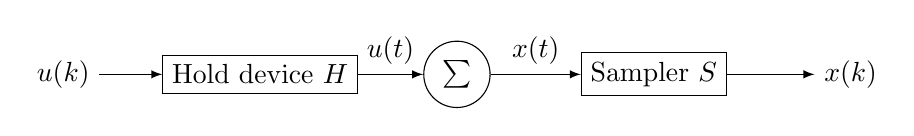
\begin{tikzpicture}[auto, node distance=2.5cm, >=latex]
    % Nodes
    \node (u) {$u(k)$};
    \node [rectangle, draw, right of=u] (H) {Hold device $H$};
    \node [circle, draw, right of=H] (sum) {$\sum$};
    \node [rectangle, draw, right of=sum] (S) {Sampler $S$};
    \node (x) [right of=S] {$x(k)$};

    % Connections with labels
    \draw [->] (u) -- (H);
    \draw [->] (H) -- node[above] {$u(t)$} (sum);
    \draw [->] (sum) -- node[above] {$x(t)$} (S);
    \draw [->] (S) -- (x);
\end{tikzpicture}
\end{center}

\begin{itemize}
    \item \(S\) is the \textbf{sampler} that samples the continuous-time state at intervals \(T\): \(x(k)=x(kT)\).  
    \item \(H\) is the \textbf{hold device} (e.g., zero-order hold) that converts the discrete input \(u(k)\) into a piecewise constant continuous-time signal \(u(t)\).  
    \item The summation block represents the \textbf{continuous-time plant} \(\dot{x}=f(x,u)\).  
    \item The discrete-time summation \(\sum_d\) combines the sampler and hold, giving the discrete evolution:
    \[
    x(k+1) = F(x(k), u(k), T) \approx f_d(x(k),u(k)).
    \]
\end{itemize}

\subsection{Case 1: LTI Plants}\index{Discretization!LTI Plants}

Consider a linear time-invariant (LTI) system:
\[
\dot{x}(t) = A x(t) + B u(t), \quad x(0) = x_0.
\]

Using the zero-order hold over the sampling interval \(T\), the solution is
\[
x((k+1)T) = e^{A T} x(kT) + \int_{0}^{T} e^{A\tau} B u((k+1)T - \tau) \, d\tau.
\]

If \(u(t)\) is piecewise constant \(u(t) = u(k)\) for \(kT \le t < (k+1)T\), the integral simplifies:
\[
\int_0^T e^{A \tau} B u(k) \, d\tau = \left(\int_0^T e^{A \tau} d\tau \right) B u(k),
\]
so the discrete-time model is
\[
\boxed{x(k+1) = e^{A T} x(k) + \left( \int_0^T e^{A \tau} d\tau \right) B u(k)}.
\]

\subsection{Case 2: Nonlinear Plants}\index{Discretization!Nonlinear Plants}

For a nonlinear system
\[
\dot{x} = f(x,u),
\]
a simple forward Euler approximation over the sampling interval \(T\) gives:
\[
\boxed{x(k+1) \approx x(k) + T f(x(k), u(k))}.
\]

This is a first-order discrete-time approximation suitable for small \(T\) and is widely used in digital control of nonlinear systems.

\section{Stability of Discrete-Time Systems}\index{Stability of Discrete-Time Systems}

\subsection{Definitions}\index{Stability of Discrete-Time Systems!Definitions}
\begin{definition}[Stability Concepts]
Consider the discrete-time system $x(k+1) = f(x(k),k)$ with equilibrium $x=0$.  
\begin{itemize}
    \item \textbf{Stable:} For every $\epsilon>0$ there exists $\delta>0$ such that
    \[
    ||x(k_0)|| < \delta \;\; \Rightarrow \;\; ||x(k)|| < \epsilon, \quad \forall k \ge k_0.
    \]
    \item \textbf{Convergent:} $x(k) \to 0$ as $k \to \infty$.
    \item \textbf{Asymptotically Stable:} The equilibrium is stable and convergent.  
    \item \textbf{Unstable:} The equilibrium is not stable.  
\end{itemize}
\end{definition}

\begin{definition}[Uniform Stability Concepts]
The equilibrium $x=0$ is said to be uniformly stable if the $\delta$ in the stability definition is independent of $k_0$.  
\begin{itemize}
    \item \textbf{Uniformly Stable:} $\delta = \delta(\epsilon)$ independent of $k_0$.  
    \item \textbf{Uniformly Convergent:} For every $\epsilon>0$, there exists $N(\epsilon)>0$ independent of $k_0$ such that
    \[
    k \ge k_0 + N(\epsilon) \;\; \Rightarrow \;\; ||x(k)|| < \epsilon.
    \]
    \item \textbf{Uniformly Asymptotically Stable (UAS):} Uniformly stable and uniformly convergent.  
    \item \textbf{Globally Uniformly Asymptotically Stable (GUAS):} Uniformly asymptotically stable with region of attraction $\mathbb{R}^n$.  
\end{itemize}
\end{definition}

\begin{definition}[Exponential Stability]
The equilibrium $x=0$ is \textbf{exponentially stable} if there exist constants $\alpha>0$, $\lambda>0$ such that
\[
||x(k)|| \leq \alpha \, ||x(k_0)|| (1-\lambda)^{k-k_0}, \quad \forall k \ge k_0, \; ||x(k_0)|| < \delta.
\]
If the inequality holds for all $x(k_0)\in\mathbb{R}^n$, the equilibrium is \textbf{globally exponentially stable}.
\end{definition}

%------------------------------------------------
\subsection{Discrete-Time Positive Definite Functions}\index{Stability of Discrete-Time Systems!Discrete-Time Positive Definite Functions}
Let $W : D \times \mathbb{Z}^+ \to \mathbb{R}$ be a scalar function, where $D \subseteq \mathbb{R}^n$ contains the origin. Assume $W(x,k)$ is continuous in $x$ for each $k$.  

\begin{definition}[Positive Semi-Definite Function]
$W(x,k)$ is \textbf{positive semi-definite} in $D$ if
\[
W(0,k) = 0, \quad W(x,k) \ge 0, \;\; \forall x\in D, k \in \mathbb{Z}^+.
\]
\end{definition}

\begin{definition}[Positive Definite Function]
$W(x,k)$ is \textbf{positive definite} if
\[
W(0,k) = 0, \quad W(x,k) > 0 \;\; \forall x \neq 0,
\]
and there exists a continuous function $V_1(x)$ with $V_1(0)=0$ such that
\[
V_1(x) \leq W(x,k), \quad \forall x \in D, k \in \mathbb{Z}^+.
\]
\end{definition}

\begin{definition}[Decrescent Function]
$W(x,k)$ is \textbf{decrescent} in $D$ if there exists a continuous function $V_2(x)$ with $V_2(0)=0$ such that
\[
W(x,k) \leq V_2(x), \quad \forall x \in D, k \in \mathbb{Z}^+.
\]
\end{definition}

\begin{definition}[Radially Unbounded Function]
$W(x,k)$ is \textbf{radially unbounded} if
\[
||x|| \to \infty \;\; \Rightarrow \;\; W(x,k) \to \infty, \quad \forall k \in \mathbb{Z}^+.
\]
\end{definition}

\begin{example}[Discrete-Time Positive Definite Function]
Consider
\[
W(x,k) = (1+0.5\cos k)\|x\|^2, \quad x\in\mathbb{R}^n, k \ge 0.
\]

\begin{itemize}
    \item \textbf{Positive semi-definite:} $W(x,k) \ge 0$.  
    \item \textbf{Positive definite:} $W(0,k) = 0$ and $W(x,k) > 0$ for $x \neq 0$.  
    \item \textbf{Decrescent:} $W(x,k) \le 1.5\|x\|^2$, take $V_2(x)=1.5\|x\|^2$.  
    \item \textbf{Radially unbounded:} As $\|x\|\to \infty$, $W(x,k)\to\infty$.  
\end{itemize}
\end{example}

%------------------------------------------------
\subsection{Stability Theorems}\index{Stability of Discrete-Time Systems!Stability Theorems}

\begin{theorem}[Lyapunov Stability Theorem for Discrete-Time Systems]
If $W:D \times \mathbb{Z}^+ \to \mathbb{R}$ is positive definite and
\[
\Delta W(x(k)) = W(x(k+1),k+1) - W(x(k),k) \le 0,
\]
then the equilibrium $x=0$ is \textbf{stable}.
\end{theorem}

\begin{theorem}[Uniform Asymptotic Stability for Discrete-Time Systems]
If $W(x,k)$ is positive definite, decrescent, and
\[
\Delta W(x(k)) < 0, \quad x\neq 0,
\]
then the equilibrium $x=0$ is \textbf{uniformly asymptotically stable}.
\end{theorem}

\begin{theorem}[Global Uniform Asymptotic Stability]
If $W(x,k)$ is positive definite, decrescent, radially unbounded, and
\[
\Delta W(x(k)) < 0, \quad x\neq 0,
\]
then the equilibrium $x=0$ is \textbf{globally uniformly asymptotically stable}.
\end{theorem}

\begin{remark}\textbf{Hierarchy of Discrete-Time Stability}
\[
\text{GUAS} \;\Rightarrow\; \text{UAS} \;\Rightarrow\; \text{Asymptotic Stability} \;\Rightarrow\; \text{Stability}.
\]
The converse implications do not hold in general.
\end{remark}
